\RequirePackage{fix-cm}
%
%\documentclass{svjour3}                     % onecolumn (standard format)
%\documentclass[smallcondensed]{svjour3}     % onecolumn (ditto)
%\documentclass[smallextended]{svjour3}       % onecolumn (second format)
\documentclass[twocolumn]{svjour3}          % twocolumn
\smartqed  % flush right qed marks, e.g. at end of proof
\usepackage{graphicx}
\usepackage[linesnumbered,ruled,vlined]{algorithm2e}
\journalname{CGI2013} % The correct name will be entered by the editor
\begin{document}

\title{Real Time Cloth Fitting for Virtual Dressing Rooms }
\subtitle{Insert your subtitle here, otherwise leave blank}
\author{Umut Gultepe  \and Ugur Gudukbay}
\institute{Bilkent University \at Ankara \and Bilkent University \at Ankara}
\date{ }% The correct dates will be entered by the editor

\maketitle

\begin{abstract}
Current cloth fitting algorithms for virtual avatars and real humans. 
\keywords{First keyword \and Second keyword \and More}
\end{abstract}

\section{Introdcution}
\label{sec:1}
Lorem ipsum dolor sit amet, consectetur adipiscing elit. Donec imperdiet tincidunt nibh quis dictum. Pellentesque eget tellus nunc. Donec semper blandit metus vel rhoncus. Nullam tincidunt enim nibh, suscipit volutpat neque. Ut eget ipsum dolor, ac semper sapien. Nunc nec rutrum nulla. Vivamus sodales auctor orci, vel bibendum leo pretium at. Fusce placerat lectus mi.

\section{Previous Works}
\label{sec:2}
Lorem ipsum dolor sit amet, consectetur adipiscing elit. Donec imperdiet tincidunt nibh quis dictum. Pellentesque eget tellus nunc. Donec semper blandit metus vel rhoncus. Nullam tincidunt enim nibh, suscipit volutpat neque. Ut eget ipsum dolor, ac semper sapien. Nunc nec rutrum nulla. Vivamus sodales auctor orci, vel bibendum leo pretium at. Fusce placerat lectus mi.

\section{Methodology}
\label{sec:3}
Objective is to acquire a set of simulation parameters from a human test-subject for a pre-modeled clothing mesh,
 which is to be displayed on a virtual avatar reflecting the body characteristics of the aforementioned subject.
  The set of parameters for the simulation include the body height and width, also the radii for the collision 
  spheres which have their centers coinciding with the joints of the virtual avatar's skeleton. 
  Body width and height are then utilized to estimate the body size of the user, collision spheres are used 
  in the dressing room simulation, to collide with the cloth particles.   
  
\subsection{Depth Map Optimization}
\label{subsec:3.1} 
The state-of the art time-of-flight cameras still provide low resolution and quality output compared to current advanced RGB systems. The quality of the input depth map is a crucial factor
on the overall performance of the system, therefore we first wish to improve the quality of the depth map by applying canonical image optimization methods.

Let us take the depth map D as a 640x480 matrix. Initially, the user pixels are
extracted by a pixel-by-pixel comparison with the user map. User map is another
acquired map from the sensor, with the same size as depth map. The value of a
pixel is set to a non-zero value if the pixel belongs to a recognized user. In
this case, we are only interested in one user, $D_1$ represents the depth pixels
of the user we are interested in, whereas $U_1$ is the bit map of the user.
Also, the non-user pixels must be filled with the mean value of the user pixels, in order to perform Gaussian filtering on the image.

\begin{equation}
D_1=(D-(D \times U_1 )) \times 1/n \times \sum\limits_{i=0}^n ((D \times U_1 )_i + d \times U_1 )
\label{eqn:patch_depth}
\end{equation}

Next, we perform Gaussian filtering on the user’s depth map, to normalize and
improve the quality of the depth map. The size and sigma parameters of the Gaussian filter will be varied in order to maximize the performance and the quality of the results. 

\begin{equation}
D_G=D_1*G
\label{eqn:gaussian_convolution}
\end{equation}

After these operations, we have a normalized and filtered depth map, which also
has better planar values (x and y) since the holes due to depth stream will be filled.

\begin{algorithm}
\dontprintsemicolon % Some LaTeX compilers require you to use \dontprintsemicolon instead
\KwIn{Raw Depth Stream From Kinect}
\KwOut{Depth Stream With Patched Holes and Gaussian Optimization }
$depth_{sum}=0$ \;
$n_{user} =0$\;
\For{i \bf{from} 0 \bf{to} $d_width$ }{
\For{j \bf{from} 0 \bf{to} $d_height$ }{
\If{$U(i,j)$} {
  $depth_{sum}=depth_{sum}+D(i,j)$\;
  $n_{user}+=1$\;
 }}}
$depth_{average}=depth_{sum}/n_{user}$ \;
\For{i \bf{from} 0 \bf{to} $d_width$ }{
\For{j \bf{from} 0 \bf{to} $d_height$ }{
\If{\bf{not}  $U(i,j)$} {
  $D(i,j)=depth_{average}$\;
 }}}
 
\For{i \bf{from} 0 \bf{to} $d_width$ }{
\For{j \bf{from} 0 \bf{to} $d_height$ }{
\If{$U(i,j)$} {
  $D(i,j)=D(i-m:i+m,j-n:j+m) * Gaussian(m,n,e)$\;
 }}}
\Return{D}
\caption{Depth Map Optimization Algorithm}
\label{algo:depth_patch}
\end{algorithm}

\subsection{Body Measurement}
\label{subsec:3.2} 

\subsection{Temporal Optimization}
\label{subsec:3.3}

\section{Experiments}
\label{sec:4}
Lorem ipsum dolor sit amet, consectetur adipiscing elit. Donec imperdiet tincidunt nibh quis dictum. Pellentesque eget tellus nunc. Donec semper blandit metus vel rhoncus. Nullam tincidunt enim nibh, suscipit volutpat neque. Ut eget ipsum dolor, ac semper sapien. Nunc nec rutrum nulla. Vivamus sodales auctor orci, vel bibendum leo pretium at. Fusce placerat lectus mi.


\section{Conclusion}
\label{sec:5}
Lorem ipsum dolor sit amet, consectetur adipiscing elit. Donec imperdiet tincidunt nibh quis dictum. Pellentesque eget tellus nunc. Donec semper blandit metus vel rhoncus. Nullam tincidunt enim nibh, suscipit volutpat neque. Ut eget ipsum dolor, ac semper sapien. Nunc nec rutrum nulla. Vivamus sodales auctor orci, vel bibendum leo pretium at. Fusce placerat lectus mi.


\begin{figure}
	\begin{center}
			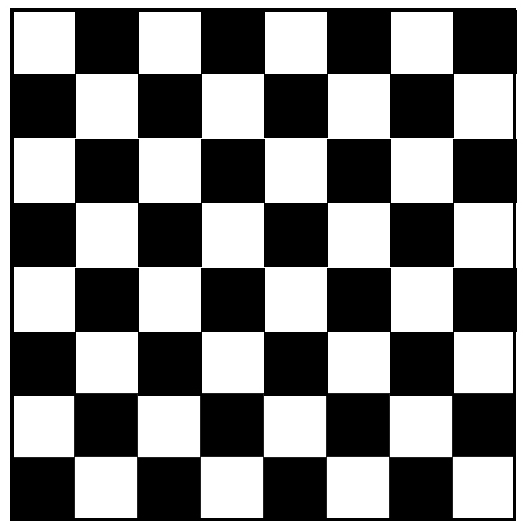
\includegraphics[width=0.9\columnwidth]{./bwgrid.jpg}
	\end{center}
	\caption{A Sample Image}
	\label{fig:1}
\end{figure}

\begin{thebibliography}{}
\bibitem{RefA}
Author, Article title, Journal, Volume, page numbers (year)
\bibitem{RefB}
Author, Book title, page numbers. Publisher, place (year)
\end{thebibliography}

\end{document}


